\chapter{Risorse, Design UI e Networking}

\section{Risorse}

Un applicazione è composta dal codice e dalle \textbf{risorse}, ossia tutto ciò che non è codice (es. file del layout in XML, pacchetti delle lingue, immagini, audio, video, ecc).
Ci sono degli ottimi motivi per utilizzare le risorse:

\begin{itemize}
\item Separare la rappresentazione dei dati (\textit{layout}) dalla gestione dei dati (\textit{logica});
\item Fornire risorse alternative per supportare le configurazioni specifiche dei dispositivi (es. lingua);
\item Ricompilare solo quando è strettamente necessario. 
\end{itemize}

\subsection{Etereogeneità dei dispositivi}

Un'applicazione Android può essere eseguita su dispositivi eterogenei con caratteristiche differenti (es. dimensioni dello schermo, lingua, tipo di tastieta, ecc). Ci sono due differenti approcci a questo problema, quello tradizionale e quello implementato in Android.
L'approccio tradizionale prevede di inserire tutte le possibilità nel codice, per cui sarà pieno di casi \emph{if-then-else}. Per questo motivo, l'applicazione deve essere ricompilata ogni volta che viene effettuata una modifica (es. cambio di layout, aggiunta di una lingua).
L'approccio utilizzato in Android prevede di separare il codice dalle risorse, usando un approccio dichiarativo basato su XML per definire le risorse stesse. Nella Figura~\ref{img:lab2-fig1} possiamo osservare un esempio di come il codice in Java venga separato dalle varie risorse.

\begin{figure}[htbp]
	\centering
	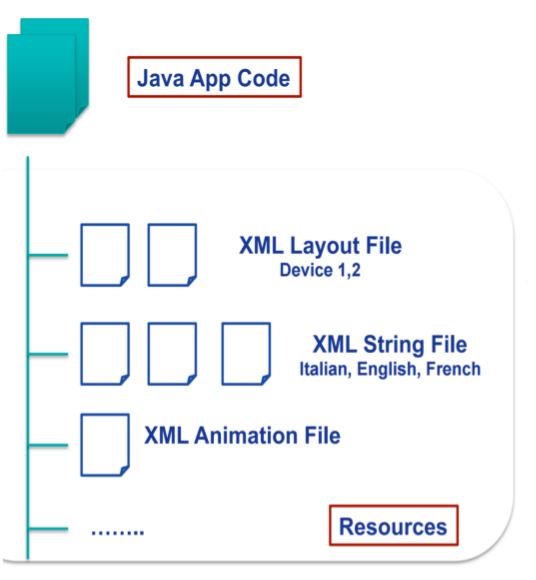
\includegraphics[width=0.8\textwidth]{lab2-fig1}
	\caption[Esempio di separazione tra codice e risorse]{Esempio di separazione tra codice e risorse.}\label{img:lab2-fig1}
\end{figure}

\subsubsection{Approccio Android}

Gli step che prevede questo metodo sono:

\begin{enumerate}
\item Usare file XML per definire
\begin{itemize}
\item Layout dell'applicazione
\item Testo usato nell'applicazione
\item Menù dell'applicazione
\item Animazioni
\item Alcuni esempi si trovano nella Figura~\ref{img:lab2-fig1}2-fig2}
\end{itemize}
\item Prevedere differenti risorse per configurazioni differenti dei vari dispositivi
\item Costruire il layout tramite file XML o l'editor
\item Definire layout XML differenti per dispositivi differenti
\item A run-time, il \textit{sistema Android} rileva la configurazione del dispositivo (\textit{locale}) e carica le risorse appropriate (in questo modo non è necessario ricompilare)
\item Aggiungere nuovi file XML per supportare nuovi dispotivi.
\end{enumerate}

\begin{figure}[htbp]
	\centering
	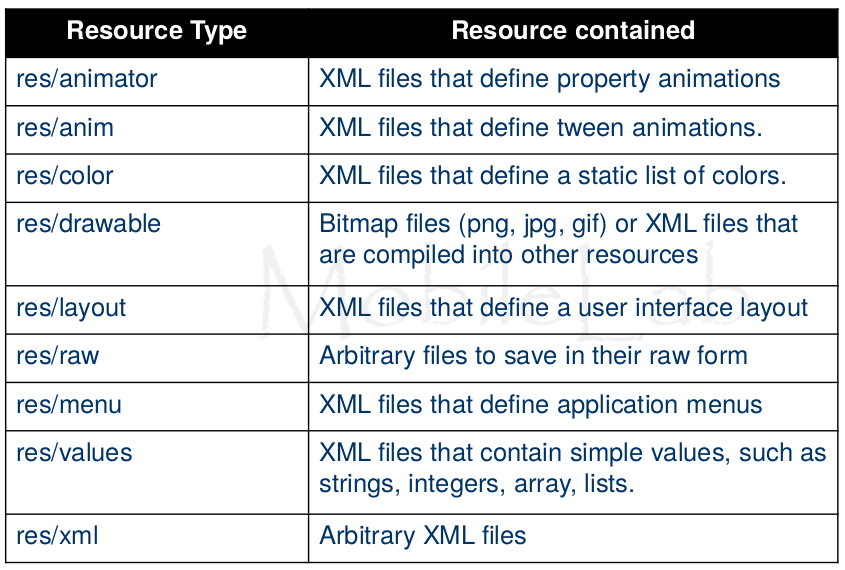
\includegraphics[width=0.8\textwidth]{lab2-fig2}
	\caption[Elenco risorse]{Un breve elenco delle risorse utilizzate sotto forma di file XML.}\label{img:lab2-fig2}
\end{figure}

Le risorse vengono definite con un approccio dichiarativo attraverso XML: ogni risorsa ha un \textit{nome/identificatore}.

%\lstinputlisting{lab2-es1.xml}

Le risorse possono essere accedute... (slide 10)

